\chapter*{LAMPIRAN}
\addcontentsline{toc}{chapter}{LAMPIRAN}
\markboth{LAMPIRAN}{LAMPIRAN}

% ============================================================================
% Helper: tampilkan gambar lampiran bila file ada; jika belum, tampilkan kotak
% placeholder agar dokumen tetap dapat dikompilasi. Ganti/isi file di folder
% gambar/ sesuai nama yang dirujuk pada tiap \lampgambar di bawah.
% Catatan: gambar lampiran TIDAK diberi \caption (tidak dinomori "Gambar X.Y"
% dan tidak masuk Daftar Gambar), sesuai konvensi bahwa isi lampiran tidak
% didaftarkan seperti gambar pada bab utama. Keterangan tetap ditampilkan
% sebagai teks biasa di bawah gambar.
% ============================================================================
\newcommand{\lampgambar}[3]{%
  \begin{figure}[H]
    \centering
    \IfFileExists{gambar/#1}%
      {\includegraphics[width=0.92\textwidth,height=0.72\textheight,keepaspectratio]{gambar/#1}}%
      {\fbox{\parbox[c][5cm][c]{0.85\textwidth}{\centering\itshape
        [#2 --- gambar belum tersedia, letakkan berkas pada folder gambar/]}}}
    \par\vspace{1ex}
    {\small #2}
  \end{figure}}

\vspace{1ex}

\noindent Lampiran berikut memuat dokumentasi perangkat keras, antarmuka
perangkat lunak, potongan kode program, dan formulir pernyataan etik
penggunaan \emph{Generative AI} yang digunakan pada penelitian ini.

% ----------------------------------------------------------------------------
\section*{Lampiran 1 \quad Skematik Rangkaian PWM AC \emph{Chopper}}
\addcontentsline{toc}{section}{Lampiran 1\quad Skematik Rangkaian PWM AC \emph{Chopper}}

\lampgambar{skematik_pwmac_chopper.png}
  {Skematik rangkaian daya PWM AC \emph{chopper}}
  {lamp:skematik-chopper}

\lampgambar{skematik_driver1.png}
  {Skematik \emph{gate driver} untuk sinyal PWM aktif}
  {lamp:skematik-driver-aktif}

\lampgambar{skematik_driver2.png}
  {Skematik \emph{gate driver} untuk sinyal PWM \emph{freewheeling}}
  {lamp:skematik-driver-freewheeling}

% ----------------------------------------------------------------------------
\section*{Lampiran 2 \quad Desain PCB}
\addcontentsline{toc}{section}{Lampiran 2\quad Desain PCB}

\lampgambar{pcb_lampiran2.png}
  {Desain \emph{layout} PCB rangkaian PWM AC \emph{chopper}}
  {lamp:pcb}

% ----------------------------------------------------------------------------
\section*{Lampiran 3 \quad Instalasi Sistem Pipa dan Pompa Air}
\addcontentsline{toc}{section}{Lampiran 3\quad Instalasi Sistem Pipa dan Pompa Air}

\lampgambar{instalasi_lampiran3.png}
  {Instalasi sistem perpipaan dan pompa air beserta empat keran}
  {lamp:sistem-pipa}

% ----------------------------------------------------------------------------
\section*{Lampiran 4 \quad Dokumentasi Pengujian}
\addcontentsline{toc}{section}{Lampiran 4\quad Dokumentasi Pengujian}

\lampgambar{pengujian_lampiran4.jpg}
  {Dokumentasi (foto) pelaksanaan pengujian sistem}
  {lamp:pengujian}

% ----------------------------------------------------------------------------
\section*{Lampiran 5 \quad Antarmuka (GUI) Akuisisi Data}
\addcontentsline{toc}{section}{Lampiran 5\quad Antarmuka (GUI) Akuisisi Data}

\lampgambar{gui_lampiran5a_tampilanawal.png}
  {Tampilan awal antarmuka (GUI) pemantauan dan akuisisi data}
  {lamp:gui-awal}

\lampgambar{gui_lampiran5b_uji.jpg}
  {Tampilan antarmuka (GUI) saat pengujian (akuisisi data berlangsung)}
  {lamp:gui-uji}

% ----------------------------------------------------------------------------
\section*{Lampiran 6 \quad Dokumentasi Pelaksanaan Pengujian}
\addcontentsline{toc}{section}{Lampiran 6\quad Dokumentasi Pelaksanaan Pengujian}

\lampgambar{lampiran_pengujian.png}
  {Dokumentasi kegiatan pelaksanaan simulasi dan pengujian sistem}
  {lamp:pengujian-kegiatan}

% ----------------------------------------------------------------------------
\section*{Lampiran 7 \quad Kode Program}
\addcontentsline{toc}{section}{Lampiran 7\quad Kode Program}

\subsection*{7.1 \quad Program \emph{Firmware} STM32 (C)}
\noindent\textit{Ditampilkan potongan kode inti (bukan program secara utuh) yang merepresentasikan implementasi utama sistem: pengaturan PWM, akuisisi sensor tekanan, dan pengendali \emph{Neural Network}.}

\vspace{1ex}
\noindent\textbf{Pengaturan frekuensi dan \emph{duty cycle} sinyal PWM}
\lstinputlisting[style=lampstyle, language=C, firstline=666, lastline=691]{kode/main.c}

\noindent\textbf{Akuisisi dan pemfilteran sensor tekanan}
\lstinputlisting[style=lampstyle, language=C, firstline=693, lastline=721]{kode/main.c}

\noindent\textbf{\emph{Forward pass} MLP 3--4--1}
\lstinputlisting[style=lampstyle, language=C, firstline=1106, lastline=1129]{kode/main.c}

\noindent\textbf{Fungsi keamanan terhadap tekanan berlebih}
\lstinputlisting[style=lampstyle, language=C, firstline=1137, lastline=1176]{kode/main.c}

\noindent\textbf{Pembaruan keputusan kendali NN}
\lstinputlisting[style=lampstyle, language=C, firstline=1181, lastline=1213]{kode/main.c}

\subsection*{7.2 \quad Program GUI Akuisisi Data (Python)}
\begin{itemize}
  \item \texttt{policy\_step(error)} --- aturan kendali sederhana untuk mode \emph{open-loop} / \emph{manual}.
  \item \texttt{class SerialWorker} --- \emph{thread} latar untuk komunikasi serial dengan STM32 (membaca dan mengirim data).
  \item \texttt{class App(tk.Tk)} --- antarmuka GUI berbasis Tkinter: panel kendali, grafik tekanan \emph{real-time}, tombol \emph{start/stop}, dan penyimpanan data ke CSV.
\end{itemize}

\noindent\textbf{Kebijakan kendali \emph{open-loop}/\emph{manual}}
\lstinputlisting[style=lampstyle, language=Python, upquote=false, firstline=55, lastline=73]{kode/pwm_ac_chopper_gui.py}

\noindent\textbf{\emph{Thread} komunikasi serial dengan STM32}
\lstinputlisting[style=lampstyle, language=Python, upquote=false, firstline=76, lastline=115]{kode/pwm_ac_chopper_gui.py}

\noindent\textbf{Pengambilan keputusan otomatis dan pencatatan data ke CSV}
\lstinputlisting[style=lampstyle, language=Python, upquote=false, firstline=681, lastline=719]{kode/pwm_ac_chopper_gui.py}

\subsection*{7.3 \quad Program Pelatihan \emph{Neural Network} (Python)}
\begin{itemize}
  \item \textbf{Arsitektur model:} MLP 3--4--1 --- 3 neuron masukan
  (\texttt{error}, \texttt{d\_error}, \texttt{duty\_percent}), 1 \emph{hidden
  layer} berisi 4 neuron dengan aktivasi \emph{tanh}, 1 neuron keluaran linear
  (memprediksi $\Delta duty$). Diimplementasikan sebagai \texttt{Pipeline}
  \texttt{scikit-learn}: \texttt{StandardScaler} $\rightarrow$
  \texttt{MLPRegressor} (\texttt{solver=lbfgs}, \texttt{alpha=1e-3},
  regularisasi $L_2$).
  \item \texttt{metrics(yt, yp)} --- menghitung RMSE, MAE, dan R$^2$ untuk
  evaluasi model pada data latih, validasi, dan uji.
  \item \texttt{carr(a, name)} --- mencetak \emph{array} terlatih (bobot,
  \emph{bias}, parameter \texttt{StandardScaler}) dalam format larik C statis,
  siap ditempel ke \texttt{main.c} untuk \emph{deployment} ke STM32.
  \item Proses utama: memuat dan menggabungkan data CSV dari seluruh episode,
  merekayasa fitur (\texttt{error}, \texttt{d\_error}, \texttt{delta\_duty}),
  membagi data latih/validasi/uji (70:10:20), melatih MLP 3--4--1, mengevaluasi
  terhadap \emph{baseline} sederhana, lalu mengekspor bobot ke STM32.
\end{itemize}

% ----------------------------------------------------------------------------
\section*{Lampiran 8 \quad Form Pernyataan Kode Etik Penggunaan \emph{Generative AI}}
\addcontentsline{toc}{section}{Lampiran 8\quad Form Pernyataan Kode Etik Penggunaan \emph{Generative AI}}

\begin{figure}[H]
  \centering
  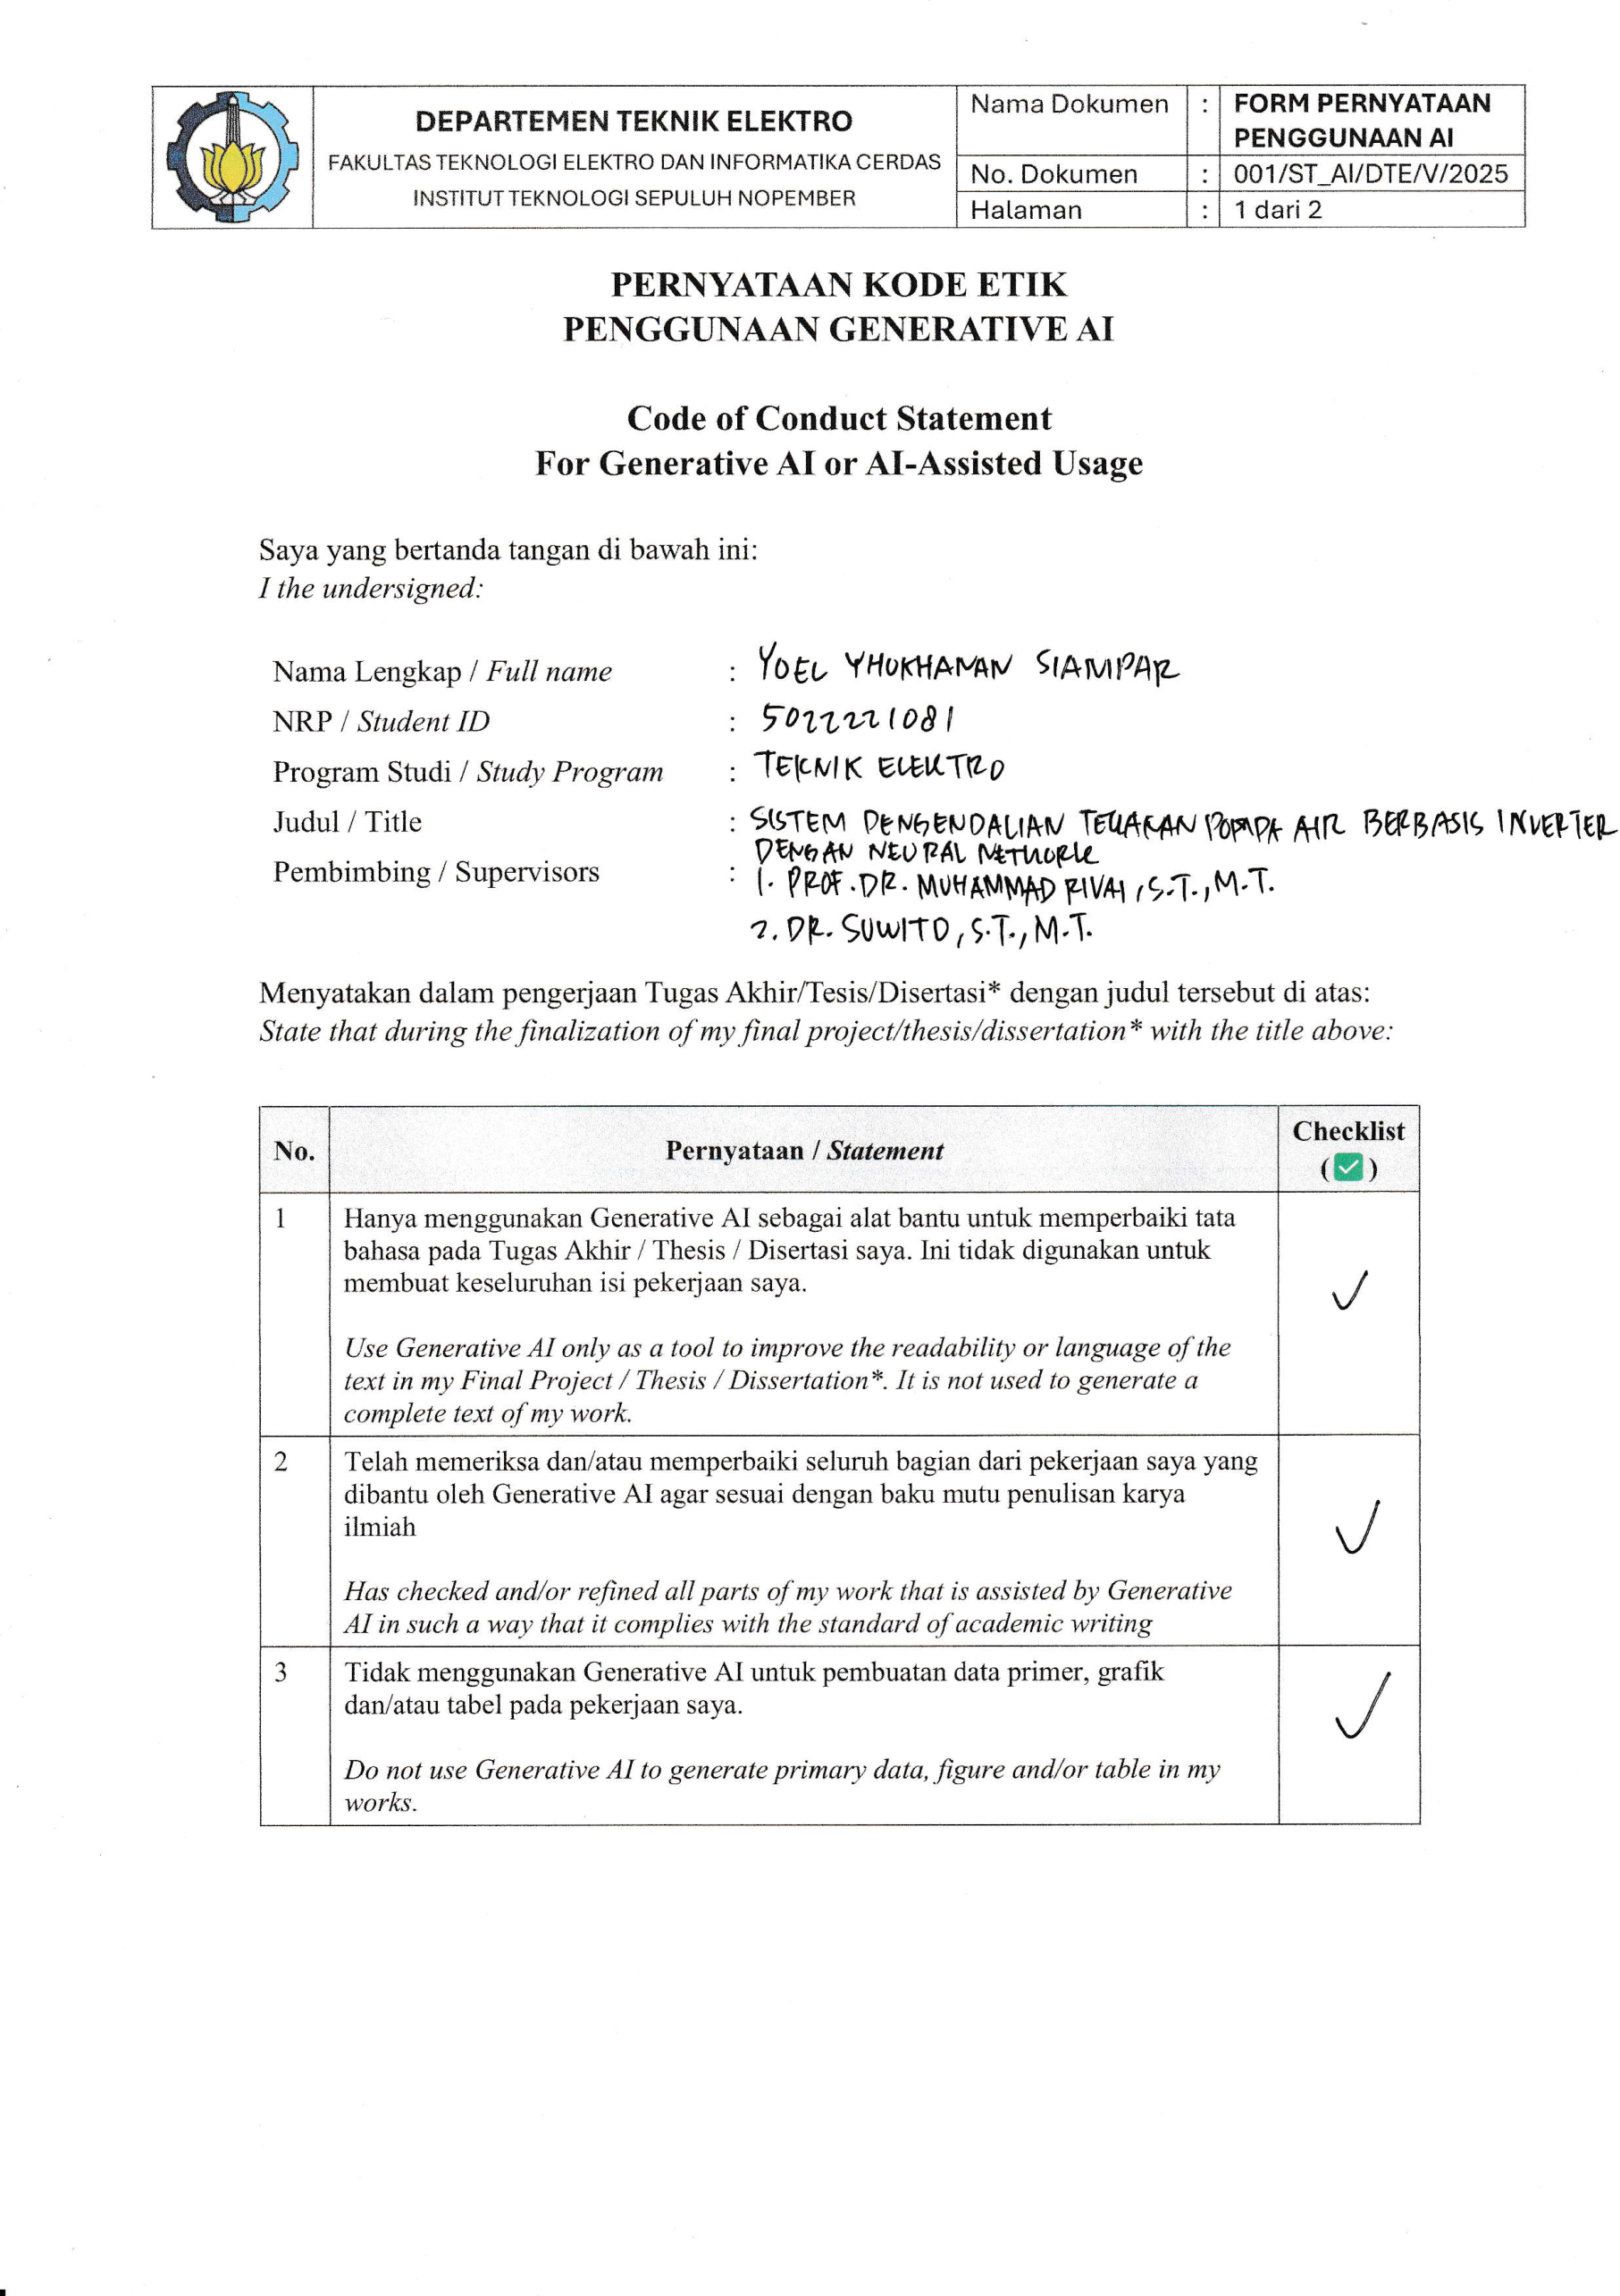
\includegraphics[width=1.0\textwidth,height=0.88\textheight,keepaspectratio]{gambar/kode_etik_ai_1.png}
\end{figure}

\clearpage
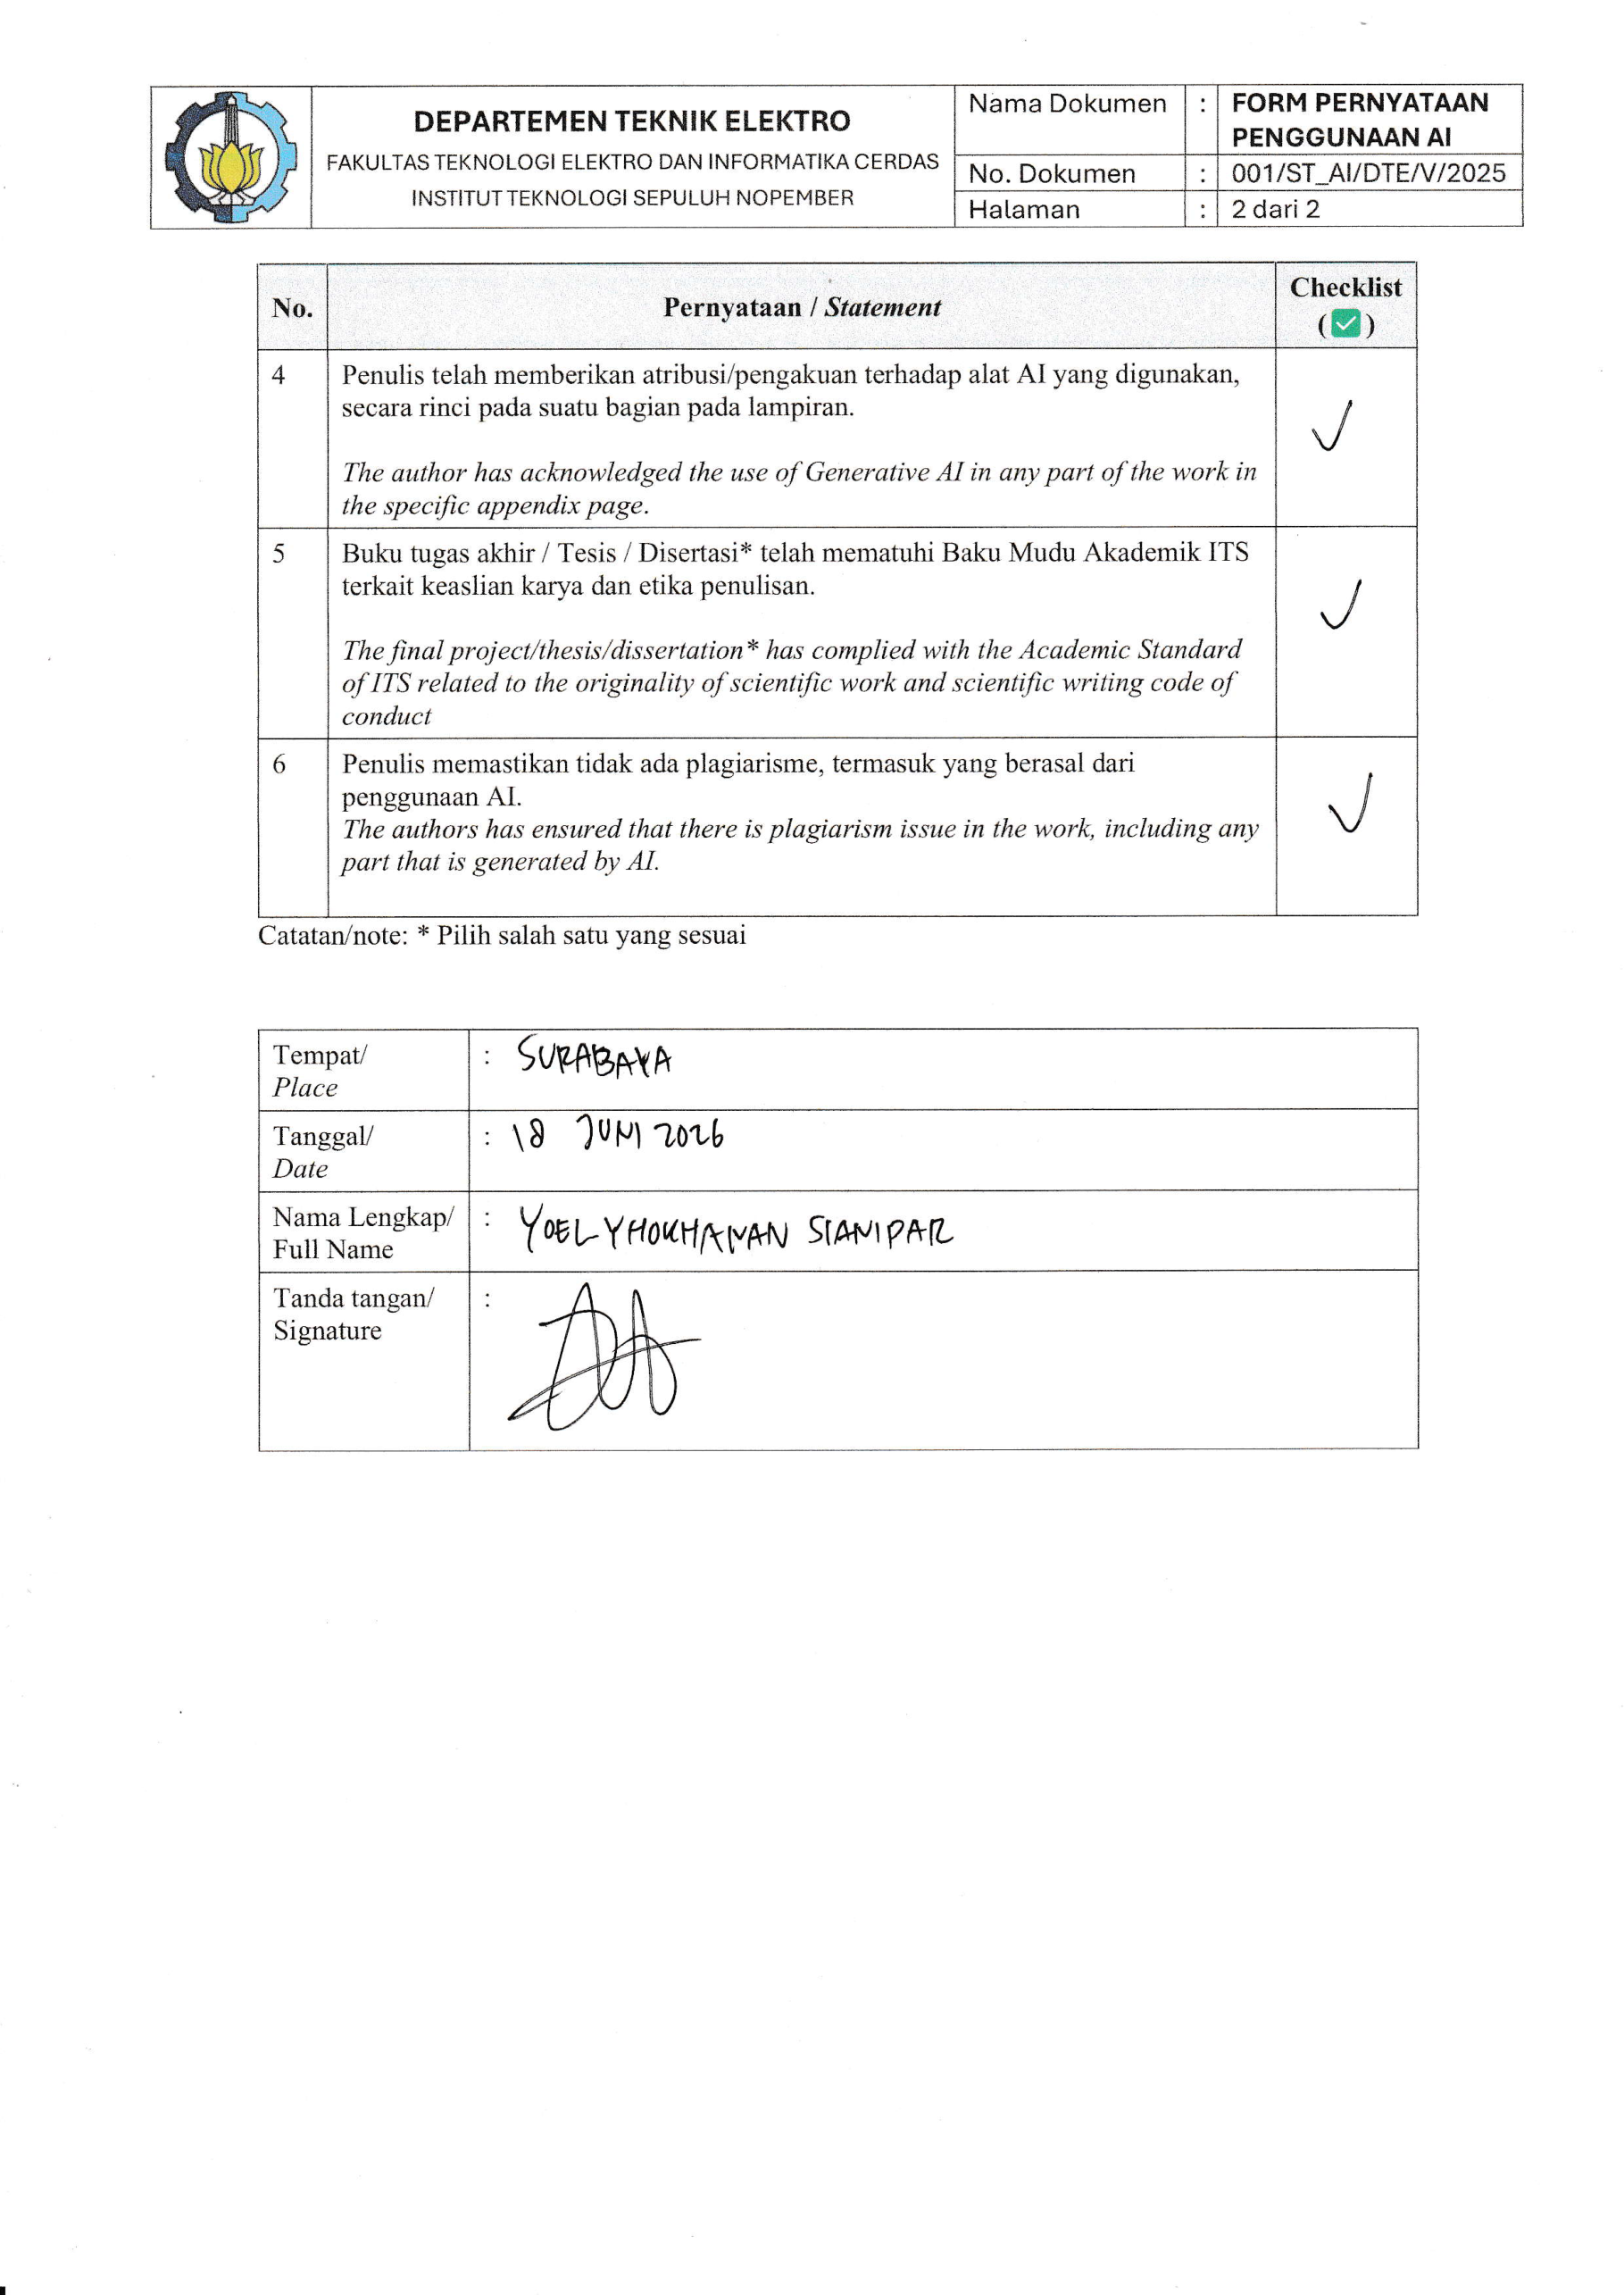
\includepdf[pages=1, pagecommand={\thispagestyle{empty}}]{gambar/kode_etik_ai_2.pdf}
